\documentclass{beamer}
\usepackage[utf8x]{inputenc}

% ggf. Pausen deaktivieren (Druckversion)
%\documentclass[handout]{beamer} % \pause deaktivieren

% Standard-Beamer verwenden
\usepackage{default}

% Konfiguration
% languages
\usepackage[ngerman,english]{babel}

% Paper layout
\usepackage[a4paper,top=30mm,right=30mm,bottom=35mm,left=30mm]{geometry}

% Math related packages
\usepackage{amsmath,amsthm,amssymb}
\usepackage{mathtools}

% typesetting (layout)
\usepackage{array}

% Enumerations
\usepackage{enumerate}

% use links for table of contents, citations, ...
\usepackage[colorlinks, linkcolor = black, citecolor = black, filecolor = black, urlcolor = blue]{hyperref} 
% markup for text
\newcommand{\defNotion}[1]{\emph{#1}} % for the defined notion in a definition
\newcommand{\TODO}[1]{\marginpar{\footnotesize{#1}}} % for todos

% reductions
\newcommand{\redmany}{\leq_{m}^{p}}

% symbols
%% sets of numbers
\newcommand{\IN}{\mathbb{N}}
%% sets of functions
\newcommand{\setOfFunctions}[1]{\mathcal{#1}}
\newcommand{\FP}{\setOfFunctions{FP}}
%% complexity classes
\newcommand{\cclass}[1]{\text{#1}}
\renewcommand{\P}{\cclass{P}} % \P is a paragraph symbol
\newcommand{\OPT}{\cclass{OPT}}
\newcommand{\NTIME}{\cclass{NTIME}}
\newcommand{\coNTIME}{\cclass{co-NTIME}}
\newcommand{\NEXP}{\cclass{NEXP}}
\newcommand{\coNEXP}{\cclass{co-NEXP}}
\newcommand{\NE}{\cclass{NE}}
\newcommand{\coNE}{\cclass{co-NE}}

% operators
%% on sets
\DeclareMathOperator{\dens}{dens}
%% on machines
\DeclareMathOperator{\runtime}{time}

% Farbschema
\usetheme{default}
\usecolortheme{default}

% Formatierung von Literaturverweisen
\setbeamertemplate{bibliography item}[text]

% Formatierung von "verdecktem" Text
\setbeamercovered{transparent}

% Anzahl der Abschnitte, die Nummeriert werden
\setcounter{secnumdepth}{5}

% Absatz-Abstand
\setlength{\parskip}{6pt}

% Formatierung von Zitaten für Theoreme
\newcommand{\rcite}[1]{\flushright\textcolor{gray}{\cite{#1}}}
\newcommand{\rciteplain}[1]{\flushright\textcolor{gray}{#1}}

% Propositions-Theorem-Umgebung
\newtheorem{proposition}[theorem]{Proposition} % Proposition numbering together with theorem

% Figure-Caption
\usepackage{caption}
\captionsetup{labelformat=empty,labelsep=none}

% Metadaten
\title[Simulation von Beweissystemen]{Simulation von Beweissystemen}
\subtitle[Bachelor Kolloquium]{Bachelor Kolloquium}
\author[N. Wisiol]{Nils Wisiol}
\institute[Informatik -- Uni Würzburg]{Lehrstuhl für Informatik IV\\Institut für Informatik\\ Julius-Maximilians-Universität Würzburg}
\date[04.06.2012]{04. Juni 2012}
\subject{Simulation von Beweissystemen}

\begin{document}

  % Titelfolie
  \maketitle

  % Inhaltsverzeichnis
  \begin{frame}
    \frametitle{Outline}
    \small
    \tableofcontents[hidesubsections]
    \normalsize
  \end{frame}
  
  % Inhalt
  \section{Einführung} 
\subsection{Beweissysteme und die $\P$-$\NP$-Frage}

\begin{frame}
  \frametitle{Die \(\P\)-\(\NP\)-Frage}
  
  \begin{quotation}
    ``If \(\P=\NP\), then the world would be a profoundly different place than we usually assume it to be. There would be no special value in `creative leaps', no fundamental gap between solving a problem and recognizing the solution once it's found. Everyone who could appreciate a symphony would be Mozart; everyone who could follow a step-by-step argument would be Gauss; everyone who could recognize a good investment strategy would be Warren Buffett.``
  \end{quotation}
  
  \rciteplain{Scott Aaronson \\ \footnotesize{\href{http://www.scottaaronson.com/}{scottaaronson.com}}}
   
\end{frame}

\begin{frame}
  \frametitle{Konsequenzen aus der Theorie der Beweissysteme für die \(\P\)-\(\NP\)-Frage}
  
  \begin{lemma}
    \(\NP \neq \coNP \implies \P \neq \NP\).
  \end{lemma}  
 
  \pause
  
  \begin{proposition} \label{prpNPcoNP}
    Es ist genau dann \(\NP\) = \(\coNP\), wenn ein polynomiell beschränktes Beweissystem für \(\TAUT\) existiert.
    \rcite{KMT03}
  \end{proposition}
  
\end{frame}

  \section{Definition} 
\subsection{Beweissysteme}

\begin{frame}
  \frametitle{Beweissysteme}
  
  \onslide<1-3> Eine \(\FP\)-Funktion \(h\) ist ein \defNotion{Beweissystem} für eine Sprache \(L\), wenn \(f(\Sigma^*) = L\). 
  \onslide<2-3> Ist \(h(w) = x\), so ist \(w\) ein \defNotion{\(h\)-Beweis} für \(x\). 
  \onslide<3-3> \(h\) ist \defNotion{polynomiell beschränkt}, wenn es ein Polynom \(p\) gibt, so dass für jedes \(x \in L\) ein \(h\)-Beweis \(w\) mit \(|w| \leq p(|x|)\) existiert. 
  
  \onslide<4-8> Sind \(h\) und \(h'\) Beweissysteme für die Sprache \(L\), 
  \onslide<5-8> und gibt es ein Polynom \(p\) und eine Funktion \(f\) 
  \onslide<6-8> so dass für alle \(h'\)-Beweise \(w\) \[ h(f(w)) = h'(w) \] 
  \onslide<7-8> mit \(|f(w)| \leq p(|w|)\) gilt, 
  \onslide<8-8> dann \defNotion{simuliert} \(h\) das Beweissystem \(h'\). 
  
  \onslide<9-10> Simuliert ein Beweissystem \(h\) für die Sprache \(L\) jedes Beweissystem der Sprache \(L\), so nennen wir es \defNotion{optimal}. 
  \onslide<10-10> Die Komplexitätsklasse aller Sprachen, die optimale Beweissysteme besitzen, sei mit \(\OPT\) bezeichnet.
\end{frame}


  \section{Beweis der Motivation} 
\subsection{Beweis von Proposition 1}

\begin{frame}
  \frametitle{Proposition 1}

  \begin{center}
   
    \(\P = \NP\)
    \onslide<2-> \(\Rightarrow \NP = \coNP\)
    \onslide<3-> \(\Leftrightarrow \TAUT \in \NP\)
    \onslide<4-5> \(\Leftrightarrow \TAUT \text{ besitzt poly. beschr. Beweissystem}\)

  \end{center}
  
  \onslide<1->
  \begin{itemize}
   \item<2> Denn \(\P = \coP\)
   \item<3> Lemma 6
   \item<4> Lemma 7
  \end{itemize}
\end{frame}

\section{Sprachen mit optimalen Beweissystemen}

\begin{frame}
  \frametitle{Sprachen mit Beweissystemen}

  \begin{itemize}
    \item<2-> \(P\) \onslide<3-> Jedes \(x \in L\) ist sein eigener Beweis
    \item<4-> \(NP\) \onslide<5-> wie oben, nur mit Trick: Nummer des berechnenden Pfades ist auch Eingabe
  \end{itemize}
\end{frame}

  \section{Hauptsatz} 
\subsection{Sprachen ohne optimales Beweissystem}

\begin{frame}
  \frametitle{Sprachen ohne optimales Beweissystem}
  
  \begin{theorem}
    Es gibt eine Sprache \(L \in \coNTIME(2^n)\), die kein optimales Beweissystem besitzt.
  \end{theorem}
\end{frame}

\subsection{Beweis}

\begin{frame}
  \frametitle{Beweisidee}

  \begin{enumerate}
   \item<1-> \(f_1, f_2, ...\): Aufzählung aller \(\FP\)-Funktionen
   \item<2-> \(L_i = 0^i10^*\) \\
              \onslide<3-> \(L_i'\) sind die Wörter aus \(L_i\), für die keine kurzen \(f_i\)-Beweise existieren \\
              \onslide<4-> \(L = \bigcup_i L_i' \in \coNTIME(2^n)\)
   \item<5-> \(L\)-Beweissystem \(f_i\): \(L_i' = L_i\), daher gibt es nur lange \(f_i\)-Beweise für \(L_i' \subset L\)
   \item<6-> Daher führt die Anname, dass \(f_i\) ein optimales Beweissystem für \(L\) ist, zum Widerspruch
  \end{enumerate}
\end{frame}

\begin{frame}
  \frametitle{Eine Aufzählung aller \(\FP\)-Funktionen}

  \begin{columns}
    \column{.7\textwidth}
      \begin{itemize}
        \item<2-> Gödel: \(M_1, M_2, ...\)
        \item<3-> \(M_1', M_2', ...\): \(M_i\) mit Wecker-Modifikation, sodass \(\runtime(M_i) \leq n^i + i\)
        \item<4-> \(f_i\): die von \(M_i\) berechnete Funktion
        \item<5-> \(n^i + i\) unbeschränkt, daher alle \(\FP\)-Funktionen
      \end{itemize}

    \column{.3\textwidth}
      \begin{figure}
        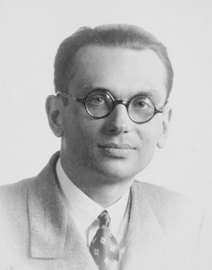
\includegraphics[width=\textwidth]{Presentation/Images/KurtGoedel.jpg}
        \caption{Kurt Gödel \\ 1906 -- 1978}
      \end{figure}
  \end{columns}
\end{frame}

\begin{frame}
  \frametitle{Konstruktion der gesuchten Sprache \(L\)}

  \begin{columns}
    \column{.2\textwidth}
      \begin{figure}
        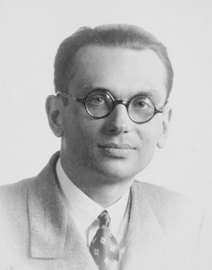
\includegraphics[width=\textwidth]{Presentation/Images/KurtGoedel.jpg}
        \caption{Kurt Gödel \\ 1906 -- 1978}
      \end{figure}

    \column{.8\textwidth}
      \begin{itemize}
        \item<1-> \(L_i = 0^i10^*\)
        \item<2-> Wähle \(x \in L_i'\), die keine kurzen \(f_i\)-Beweise haben
                  \[L_i' = \{ x \in L_i : \forall_{y \in \Sigma^*} |y|^{2i} \leq 2^{|x|} \implies f_i(y) \neq x \}\]
        \item<3-> Vereinigung
                  \[L = \bigcup_{i>0} L_i' \]
      \end{itemize}
  \end{columns}
\end{frame}

\begin{frame}
  \frametitle{\(L\) liegt in \(\coNTIME(2^n)\)}

  Betrachte Komplexität des Komplements
  
  \begin{itemize}
   \item<2-> \(L \in \coNTIME(2^n) \Leftrightarrow \overline{L} \in \NTIME(2^n)\)
   \item<3-> \(\overline{L} = \) \onslide<4-> \( \overline{ \bigcup_{i>0} L_i' } = \) \onslide<5-> \( \bigcap_{i>0} \overline{L_i'}\)
   \item<6-> zu zeigen: \( \bigcap_{i>0} \overline{L_i'} \in \NTIME(2^n)\)
  \end{itemize}

  \onslide<6->
  
  \(\overline{L_i'} = \{ x \in \Sigma^* : \alert<8-9>{ x \notin L_i } \vee \left( \alert<11>{ \exists_{y \in \Sigma^*} \left( |y|^{2i} \leq 2^{|x|} \right) } \wedge \alert<13>{ \left( f_i(y) = x \right) } \right)  \}\)

  \onslide<7-> Sei dazu \(x\) beliebiges Wort.

  \begin{itemize}
   \item<8-> Prüfe, ob \(x\) in irgendeinem \(L_i\): \onslide<9-> \alert<9>{falls nicht, dann \(x \in \overline{L}\) }
   \item<10-> Wählte \(i^*\) so, dass \(x \in L_{i^*}\)
   \item<11-> \alert<11>{für jedes \(y\) mit \(|y|^{2i} \leq 2^{|x|}\)}: \onslide<12-> berechne \(f_{i^*}(y)\). \onslide<13-> \alert<13>{Genau falls \(f_{i^*}(y) = x\), dann \(x \in \overline{L}\).}
  \end{itemize}

  \onslide<14>
\end{frame}


\begin{frame}
  \frametitle{Eigenschaft von Beweissystemen für \(L\)}

  Erinnerung: \(L_i' = \{ x \in L_i : \forall_{y \in \Sigma^*} |y|^{2i} \leq 2^{|x|} \implies f_i(y) \neq x \}\)
  
  \begin{itemize}
   \item<2-> jedes Beweissystem für \(L\) ist ein \(f_i\)
   \item<3-> für dieses ist \(L_i = L_i'\)
  \end{itemize}

  \begin{proof}
    \begin{itemize}
      \item<4-> angenommen, es gibt ein \(x = 0^i1z \in L_i\) das nicht in \(L_i'\) liegt
      \item<5-> dann gibt es \(y\) mit \(y^{2i} \leq 2^{|x|}\) und \(f_i(y) = x\)
      \item<6-> folglich \(x \in L_i'\) und daher \(x \in L\)
    \end{itemize}
  \end{proof}
\end{frame}

\begin{frame}
  \frametitle{Widerspruch zur Existenz von optimalen Beweissystemen für \(L\)}

  \begin{itemize}
   \item<1-> Sei \(f_i\) optimales Beweissystem für \(L\)
   \item<2-> Sei
         \(g(bx) =
           \begin{cases}
             f_i(x) & (b=0) \\
             x      & (b = 1 \text{ and } x=0^i10^* \in L_i = L_i') 
           \end{cases}\)
   \item<3-> \(g\) ist Beweissystem für \(L\)
   \item<4-> \(f_i\) ist optimal, also ex. \(f^*\), Überführen von Beweisen: \(f_i(f^*(x)) = g(x)\), polynomiell beschränkt: \(|f^*(x)| \leq p(|x|)\)
   \item<5-> in \(L_i\) gibt es ein \(x\), so dass \(|f^*(x)| \leq p(|x|) \leq p(|x|)^{2i} \leq 2^{|x|}\).
   \item<6-> Definition von \(L_i'\): \(f_i(f^*(x)) \neq x\)
  \end{itemize}

\end{frame}


  \section{Folgerungen} 
\subsection{Dünne Sprachen ohne Beweissystem}

\begin{frame}
  \frametitle{Dünne Sprachen ohne Beweissystem}
\end{frame}

  \section{Zusammenfassung} 
\subsection{Zusammenfassung}

\begin{frame}
  \frametitle{Zusammenfassung}
\end{frame}

  
  % Literaturverzeichnis
  \section{Literatur}

\begin{frame}[allowframebreaks]
  \frametitle{Literatur}    
  \begin{thebibliography}{KMT03}

    \bibitem[AB09]{AB09}
    Sanjeev Arora and Boaz Barak, \emph{Computational complexity: A modern
      approach}, 1st ed., Cambridge University Press, New York, NY, USA, 2009.

    \bibitem[Coo71]{C71}
    Stephen~A. Cook, \emph{The complexity of theorem-proving procedures},
      Proceedings of the third annual ACM symposium on Theory of computing (New
      York, NY, USA), STOC '71, ACM, 1971, pp.~151--158.

    \bibitem[CR79]{CR79}
    Stephen~A. Cook and Robert~A. Reckhow, \emph{The relative efficiency of
      propositional proof systems}, Journal of Symbolic Logic \textbf{44} (1979),
      36--50.

    \bibitem[For09]{F09}
    Lance Fortnow, \emph{The status of the {P} versus {NP} problem}, Commun. ACM
      \textbf{52} (2009), no.~9, 78--86.

    \bibitem[KM00]{KM00}
    Johannes K\"{o}bler and Jochen Messner, \emph{Is the standard proof system for
      {SAT} p-optimal?}, Proceedings of the 20th Conference on Foundations of
      Software Technology and Theoretical Computer Science (London, UK, UK), FST
      TCS 2000, Springer-Verlag, 2000, pp.~361--372.

    \bibitem[KMT03]{KMT03}
    Johannes K\"{o}bler, Jochen Messner, and Jacobo Tor\'{a}n, \emph{Optimal proof
      systems imply complete sets for promise classes}, Inf. Comput. \textbf{184}
      (2003), no.~1, 71--92.

    \bibitem[KP89]{KP89}
    Jan Kraj\'{\i}cek and Pavel Pudl{\'a}k, \emph{Propositional proof systems, the
      consistency of first order theories and the complexity of computations}, J.
      Symb. Log. \textbf{54} (1989), no.~3, 1063--1079.

    \bibitem[Mes99]{Mes99}
    Jochen Messner, \emph{On optimal algorithms and optimal proof systems},
      Proceedings of the 16th annual conference on Theoretical aspects of computer
      science (Berlin, Heidelberg), STACS'99, Springer-Verlag, 1999, pp.~541--550.

    \bibitem[Pap94]{Pap94}
    Christos~H. Papadimitriou, \emph{Computational complexity}, Addison-Wesley,
      1994.

  \end{thebibliography}

\end{frame}

\begin{frame}[allowframebreaks]
  \frametitle{Bildquellen}

  \begin{itemize}
   \item Kurt Gödel: Wikipedia, \texttt{\href{https://de.wikipedia.org/w/index.php?title=Datei:Kurt_g\%C3\%B6del.jpg\&filetimestamp=20110724092213}{de.wikipedia.org}}
  \end{itemize}  
\end{frame}

  
\end{document}